\chapter{Zahlenfolgen}
Sei $X$ ein metrischer Raum.
\begin{definition}{Folgen}
	Eine \emph{Folge} ist eine Abbildung $\N\rightarrow X$, so dass jedem Element $n\in\N$ ein Element $a_n\in X$ zugeordnet wird.

	Wir schreiben oft auch $(a_n)_{n\in\N}, (a_n) \text{ oder auch einfach } a_n$
	für eine Folge.

	Die Elemente $a_n$ werden auch die Glieder der Folge oder Folgenglieder genannt.
\end{definition}
\paragraph{Beispiel:}
\begin{multicols}{2}
	Sei $(a_n)_{n\in\N}$ die Folge definiert durch $a_n=\frac{1}{n}$. Dann ist $(a_n)$ die Folge der Kehrwerte der natürlichen Zahlen.\\
	Jeder weiß, dass die Folge $a_n=\frac 1 n$ gegen Null geht, aber was bedeutet das eigentlich genau?
	\columnbreak
\begin{center}
	\begin{tikzpicture}[scale=1.5]
		\draw[->] (0,0) -- (4.2,0) node[right] {$n$};
		\draw[->] (0,0) -- (0,1.2) node[above] {$a_n$};

		\foreach \x/\y in {0.5/1,1/0.5,1.5/0.333,2/0.25,2.5/0.2,3/0.166,3.5/0.143,4/0.125}
			\draw (\x,\y) node[draw=red, fill=red, minimum size=2pt, inner sep=0pt, circle]  {};

		\foreach \x/\y in {0.5/1,1/2,1.5/3,2/4,2.5/5,3/6,3.5/7,4/8}
			\draw (\x, 0) node[draw=black, fill=none, minimum width=0pt, minimum height=2.6pt, inner sep=0pt, label={below:\y}] {};
	\end{tikzpicture}
\end{center}
\end{multicols}

\section{Konvergenz von Zahlenfolgen}
	\begin{definition}{Konvergenz einer Folge}
		\vspace*{-2em}
		\begin{multicols}{2}
		Die Folge $(a_n)_{n\in\N}$ aus dem metrischen Raum $X$ konvergiert gegen das Element $a\in X$, falls es zu jedem $\epsilon>0$ einen Index $n_0\in\N$ gibt, so dass gilt:
		\begin{equation*}
			a_n\in K_\epsilon(a) \quad\forall n\geq n_0
		\end{equation*}
		In diesem Fall heißt $a$ der Grenzwert oder auch Limes der Folge $(a_n)$ und man schreibt
		\begin{equation*}
			\lim\limits_{n\to\infty}(a_n),\ \lim (a_n),\ a_n\rightarrow a
		\end{equation*}
		\columnbreak
		\begin{center}
			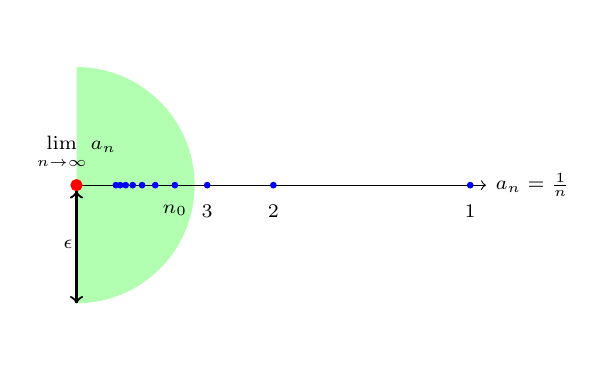
\begin{tikzpicture}
				\begin{scope}
					\clip (0,-2) rectangle (2,2);

					\draw[fill=green, opacity=0.3, draw=none] (0,0) circle (1.5);
				\end{scope}

				\draw[->] (0,0) -- (5.2,0) node[right] {\scriptsize$a_n=\frac1n$};

				\draw (0,0) node (lim) [draw=red, fill=red, minimum size=4pt, inner sep=0pt, circle, label={above:{\scriptsize$\lim\limits_{n\to\infty} a_n$}}]  {};

				\foreach \x in {5,2.5,1.66,1.25,1,0.833,0.714,0.625,0.555,0.5}
				\draw (\x,0) node[draw=blue, fill=blue, minimum size=2pt, inner sep=0pt, circle]  {};

				\draw[->, thick] (lim) to (0,-1.5);
				\draw[->, thick] (0,-1.5) to (lim);

				\draw (0.2,-0.75) node[draw=none, label={left:\scriptsize$\epsilon$}] {};
				\draw (1.25,0) node[draw=none, fill=none, label={below:\scriptsize$n_0$}] {};

				\draw (5,0) node[draw=none, fill=none, label={below:\scriptsize1}] {};
				\draw (2.5,0) node[draw=none, fill=none, label={below:\scriptsize2}] {};
				\draw (1.66,0) node[draw=none, fill=none, label={below:\scriptsize3}] {};
			\end{tikzpicture}
		\end{center}
	\end{multicols}
\end{definition}



\paragraph{Alternative Beschreibung der Konvergenz}
\begin{itemize}
	\item Eine Folge $(a_n)_{n\in\N}$ in einem metrischen Raum $X$ konvergiert gegen $a\in X$, falls gilt:
	\begin{equation*}
		\forall\epsilon>0\enspace \exists n_0\in\N\enspace \forall n\geq n_0 \ :\ \varrho(a_n,a)<\epsilon
	\end{equation*}
	\item Eher eine Umschreibung: $(a_n)_{n\in\N} \rightarrow a \Leftrightarrow \varrho(a_n,a)\rightarrow 0$
\end{itemize}

\paragraph{Beispiele:}
\begin{itemize}
	\item Die Folge $a_n=\frac 1 n$ im metrischen Raum $\R$ konvergiert gegen $0$. Dies lässt sich anhand der Definition beweisen:

	Sei $\epsilon>0$

	Zu zeigen ist, dass es einen Index (eine natürliche Zahl) $n_0\in\N$ gibt, so dass:
	\begin{equation*}
		\varrho(a_n,0)=\frac 1 n - 0=\frac 1 n <\epsilon
	\end{equation*}
	für alle $n\geq n_0$ gilt. $\sfrac 1 n<\epsilon$ ist äquivalent zu $n>\sfrac 1 \epsilon$.

	Wir wählen daher $n_0$ als irgendeine natürliche Zahl, die größer als $\sfrac 1 \epsilon$ ist.

	Dann gilt $|\sfrac 1 n-0|=\sfrac 1 n<\epsilon$ \hfill $\Box$

	\item Eine Folge muss nicht konvergieren, z.B. hat $b_n=n$ \emph{keinen} Grenzwert. Man nennt die Folge $(b_n)$ \emph{divergent}.

	\item Sei $X=\R$ und die Folge $(c_n)$ definiert durch $c_n=(-1)^n$. Diese Folge hat ebenso keinen Grenzwert, ist also divergent. Man nennt die Folge $(c_n)$ außerdem \emph{alternierend}.
\end{itemize}


Manchmal (nicht in dieser Vorlesung) sagt man auch $b_n\underset{n\rightarrow \infty}{\longrightarrow}\infty$ (uneigentliche Konvergenz)

\paragraph{Bemerkung:}
Eine Folge $(a_n)$ in einem metrischen Raum konvergiert genau dann gegen $a$, wenn $\varrho(a_n,a)\rightarrow 0$. Es muss aber nicht gelten, dass $\varrho(a_n,a)$ monoton gegen Null geht.\\
Zum Beispiel konvergiert die Folge
\begin{equation*}
	a_n=\frac{1}{n+1+(-1)^n} \rightsquigarrow 1,\sfrac14,\sfrac13,\sfrac16,\sfrac15,\sfrac18,\sfrac17,\ldots
\end{equation*}
gegen Null.


\begin{satz}{Eindeutigkeit des Grenzwerts}
	Der Grenzwert einer konvergenten Folge in einem metrischen Raum ist eindeutig bestimmt.
\end{satz}
\beweis
Sei $(a_n)_{n\in\N}$ eine Folge in $X$ und seien $a,b\in X$ Grenzwerte von $(a_n)$. Wir nehmen $a\neq b$ an.\\
Sei $\delta=\varrho(a,b)$ der Abstand der beiden Punkte $a$ und $b$. Wir zeigen: $K_{\sfrac{\delta}{2}}(a)\cap K_{\sfrac{\delta}{2}}(b)=\emptyset$.\\
Angenommen, es läge ein Punkt $P$ in dieser Schnittmenge, dann gilt:
\begin{equation*}
	\varrho(a,P)<\frac\delta2 \text{ und } \varrho(b,P)<\frac\delta2
\end{equation*}
Nach der Dreiecksungleichung gilt:
\begin{align*}
	\varrho(a,b)\leq \varrho(a,P) + \varrho(b,P) < \frac\delta2 + \frac\delta2 = \delta
\end{align*}
Widerspruch wegen $\varrho(a,b)=\delta$.\\
Wegen $(a_n)\rightarrow a$ gibt es ein $n_0\in\N$ so, dass $a_n\in K_{\sfrac\delta2}$ für alle $n\geq n_0$ gilt.\\
Damit gilt aber da $K_{\sfrac{\delta}{2}}(a)$ und $K_{\sfrac{\delta}{2}}(b)$ disjunkt sind, dass $a_n\not\in K_{\sfrac{\delta}{2}}(b)$ für alle $n\geq n_0$.\\
Widerspruch zu $a_n\rightarrow b$

\begin{definition}{Beschränktheit von Folgen}
	Eine Folge $(a_n)$ in einem metrischen Raum $X$ ist beschränkt, falls es ein $x_0\in X$ und ein $R>0$ gibt, so dass $a_n\in K_R(x_0)$ für alle $n\in N$ gilt.
\end{definition}
\begin{satz}{Konvergenz und Beschränktheit}
	Konvergente Folgen sind beschränkt.
\end{satz}
\beweis
Sei $a$ der Grenzwert der Folge und $r>0$ eine positive Zahl.

Dann gibt es ein $n_0\in\N$, so dass für alle $n\geq n_0$ $a_n\in K_r(a)$ gilt.

Es gibt aber nur endlich viele Indizes ($1,\ldots,n_0-1$), deren Folgenglieder eventuell außerhalb dieser Kugelumgebung $K_r(a)$ liegen.

Wähle also am Ende die Schranke $R$ als das Maximum $R=\mathrm{max}(\varrho(a_1,a),\ldots,\varrho(a_{n_0-1},a),r)$. Damit liegt $a_n$ für alle $n\in\N$ unter der Schranke $R$.
